%!TEX root = main.tex

El curso de Introducción al Análisis Real es uno de los más pesados en la carrera de matemáticas y los estudiantes carecen casi que de toda ayuda (no hay monitorias y los espacios en clase a veces son insuficientes), por este motivos decidimos hacer este solucionario de las notas de Introducción al Análisis Real de los profesores Leonardo Rendón y Serafín Bautista, esto más que un solucionario es una guía de lectura de las notas, aquí encontrarás muchos delos conceptos o ideas del curso desde un punto de vista más de estudiante que ha sufrido esa materia y que sabe lo compleja que puede llegar a ser.\\

Esperamos que las soluciones de los ejercicios que aportamos acá sirvan de guía para entender los conceptos y mecanismos que se deben usar para atacar este tipo de problemas.\\

Muchos éxitos - mmanosalva y eochoaq

\section{Algunos ejercicios al lector: }

\begin{itemize}[leftmargin=*]
    \item [✎] Probar que $(\mathbb{R}^n,d_1)$ y $(\mathbb{R}^n,d_{\infty})$ son espacios métricos.\\

    \begin{proof}
        $\bullet$ Sean $p,q \in \mathbb{R}^n$, tenemos que:

        $$d_1(p,q)=\sum_{k=1}^n|p_k-q_k|$$

        Luego como $|p_k-q_k|\geq 0 $, $d_1(p,q)\geq 0$ (estamos sumando valores positivos). Ahora si $d_1(p,q)=0$, como $|p_k-q_k|\geq 0$ entonces $|p_k-q_k|=0$ para todo $k$, luego $p_k=q_k$ para todo $k$, es decir $p=q$, además note que 

        $$d_1(p,q)=\sum_{k=1}^n|q_k-p_k|=d_1(q,p)$$

        Esto ya que $|p_k-q_k|=|q_k-p_k|$, Ahora veamos la desigualdad triangular.

            \begin{align*}
                d_1(p,q)&=\sum_{k=1}^n|p_k-q_k|\\
                &=\sum_{k=1}^n|p_k-q_k+r_k-r_k|\\
                &\leq \sum_{k=1}^n|p_k-r_k|+\sum_{k=1}^n|r_k-q_k|=d_1(p,r)+d_1(r,q)
            \end{align*}
            
            $\bullet$ Nuevamente tomamos $p,q \in \mathbb{R}^n$, tenemos que:

        $$d_{\infty}(p,q)=\max_{1\leq k\leq n}|p_k-q_k|$$

        como $|p_k-q_k|\geq 0$ pues es claro que el máximo será mayor igual que 0 y por tanto $d_{\infty}(p,q)\geq 0$. Como $|p_k-q_k|=|q_k-p_k|$:

         $$d_{\infty}(p,q)=\max_{1\leq k\leq n}|q_k-p_k|=d_{\infty}(q,p)$$

         Ahora si $max_{1\leq k \leq n} |q_k-p_k|=0$, $|p_k-q_k|=0$ para todo $k$ (si el máximo el 0 los demás también por definición de máximo) y como $|p_k-q_k|=0$ para todo $k$, pues $p_k=q_k$ para todo k, es decir $p=q$. Veamos la desigualdad triangular.

            \begin{align*}
                d_{\infty}(p,q)&=\max_{1\leq k\leq n}|p_k-q_k|\\
                &=\max_{1\leq k\leq n}|p_k-q_k+r_k-r_k|\\
                &\leq \max_{1\leq k\leq n}|p_k-r_k|+\max_{1\leq k\leq n}|r_k-q_k|\\
                &\leq d_{\infty}(p,r)+d_{\infty}(r,q)
            \end{align*}
        
    \end{proof}

 

    \item[✎]Sea $X$ un conjunto no vacío y $f: X \rightarrow \mathbb{R}$. Diremos que $f$ es una función acotada si existe $k>0$ tal que para todo $x \in X$ se tiene $|f(x)| \leq k$. Consideremos el conjunto $B(X)=\{f: X \rightarrow \mathbb{R}: f$ es acotada $\}$. Definamos:

        $$
        \begin{aligned}
        d: B(X) \times B(X) & \rightarrow \mathbb{R} \\
        (f, g) & \mapsto d(f, g)
        \end{aligned}
        $$

        donde $d(f, g)=\sup \{|f(x)-g(x)|: x \in X\}=\sup _{x \in X}|f(x)-g(x)|$. Entonces $(B(X), d)$ es un espacio métrico.\\

        \begin{proof}
            Es inmediato que $d(f,g)\geq 0$ por definición de supremo y porque $|f(x)-g(x)|\geq 0$. Como $|f(x)-g(x)|=|g(x)-f(x)|$, entonces también se tiene que $d(f,g)=d(g,f)$.

            Tenemos que $|f(x)-g(x)|\geq 0$, luego por definición de supremo si $\sup_{x \in X}|f(x)-g(x)|=0$, entonces $|f(x)-g(x)|=0$ para todo $x\in X$, así $f=g$, o sea si $d(f,g)=0$, entonces $f=g$. Veamos ahora la desigualdad triangular ☠☠☠☠☠:
            \begin{align*}
                d(f,g)&=\sup_{x\in X}|f(x)-g(x)|\\
                &=\sup_{x\in X}|f(x)-g(x)+h(x)-h(x)|\\
                &\leq \sup_{x\in X}|f(x)-h(x)|+|h(x)-g(x)|\\
                &=\sup_{x\in X}|f(x)-h(x)|+\sup_{x\in X}|h(x)-g(x)|\\
                &=d(f,h)+d(h,g)
            \end{align*}

            Esto ya que $\sup (A+B)=\sup(A)+\sup (B)$\\
            
        \end{proof}

        \item[✎] Dado $(E, d)$ un espacio métrico, toda bola abierta es un conjunto abierto. En efecto, dados $B_E(p, r)$ (con $r>0$ y $\left.p \in E\right)$ y $q \in B_E(p, r)$, tomamos $r^{\prime}=r-d(p, q)$ de donde se tiene que $B_E\left(q, r^{\prime}\right) \subset B_E(p, r)$ (verifique esta contenencia como ejercicio).

       \begin{basedtikz}
       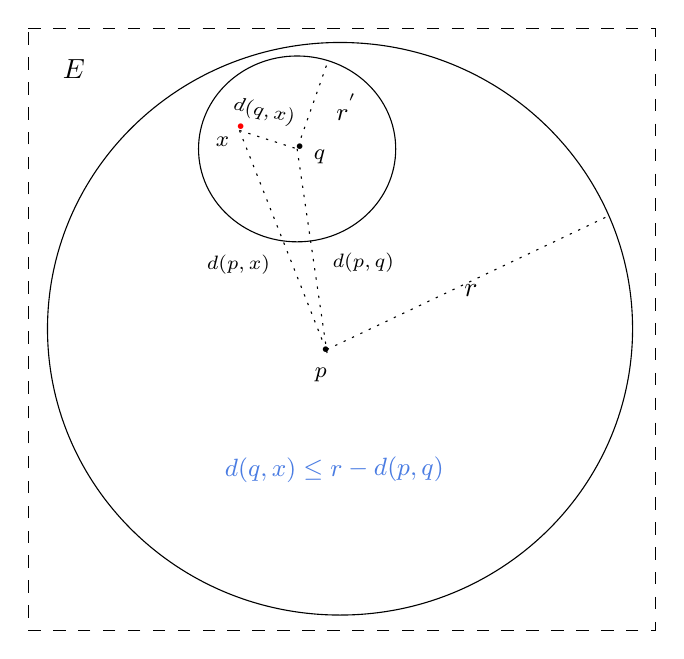
\begin{tikzpicture}[x=0.75pt,y=0.75pt,yscale=-1,xscale=1]
%uncomment if require: \path (0,472); %set diagram left start at 0, and has height of 472

%Shape: Rectangle [id:dp36732556175622055] 
\draw  [dash pattern={on 4.5pt off 4.5pt}] (158.57,81.29) -- (460.57,81.29) -- (460.57,371.29) -- (158.57,371.29) -- cycle ;
%Shape: Ellipse [id:dp4665256155664408] 
\draw   (167.85,226.09) .. controls (167.85,149.91) and (230.95,88.15) .. (308.79,88.15) .. controls (386.63,88.15) and (449.74,149.91) .. (449.74,226.09) .. controls (449.74,302.27) and (386.63,364.02) .. (308.79,364.02) .. controls (230.95,364.02) and (167.85,302.27) .. (167.85,226.09) -- cycle ;
%Straight Lines [id:da9766682347288755] 
\draw  [dash pattern={on 0.84pt off 2.51pt}]  (436.62,172.45) -- (301.2,236.7) ;
%Shape: Ellipse [id:dp01457511604137074] 
\draw   (240.62,139.43) .. controls (240.62,114.7) and (261.89,94.66) .. (288.12,94.66) .. controls (314.35,94.66) and (335.62,114.7) .. (335.62,139.43) .. controls (335.62,164.16) and (314.35,184.2) .. (288.12,184.2) .. controls (261.89,184.2) and (240.62,164.16) .. (240.62,139.43) -- cycle ;
%Straight Lines [id:da776417097753616] 
\draw  [dash pattern={on 0.84pt off 2.51pt}]  (302.22,99.3) -- (288.12,139.43) ;
%Straight Lines [id:da7683663505583478] 
\draw  [dash pattern={on 0.84pt off 2.51pt}]  (260.35,130.54) -- (300.82,233.1) ;
%Straight Lines [id:da24390474713752863] 
\draw  [dash pattern={on 0.84pt off 2.51pt}]  (260.35,130.54) -- (288.12,139.43) ;
%Straight Lines [id:da17965772530026092] 
\draw  [dash pattern={on 0.84pt off 2.51pt}]  (288.12,139.43) -- (302.59,238.19) ;

% Text Node
\draw (367.41,203.72) node [anchor=north west][inner sep=0.75pt]   [align=left] {$\displaystyle r$};
% Text Node
\draw (283.92,135.63) node [anchor=north west][inner sep=0.75pt]  [font=\Huge] [align=left] {.};
% Text Node
\draw (296.76,233.66) node [anchor=north west][inner sep=0.75pt]  [font=\Huge] [align=left] {.};
% Text Node
\draw (305.8,111.43) node [anchor=north west][inner sep=0.75pt]  [font=\small] [align=left] {$\displaystyle r^{'}$};
% Text Node
\draw (255.65,126.25) node [anchor=north west][inner sep=0.75pt]  [color={rgb, 255:red, 255; green, 0; blue, 0 }  ,opacity=1 ] [align=left] {{\Huge .}};
% Text Node
\draw (295.38,243.81) node [anchor=north west][inner sep=0.75pt]  [font=\footnotesize] [align=left] {$\displaystyle p$};
% Text Node
\draw (294.91,138.69) node [anchor=north west][inner sep=0.75pt]  [font=\footnotesize] [align=left] {$\displaystyle q$};
% Text Node
\draw (247.76,132.33) node [anchor=north west][inner sep=0.75pt]  [font=\footnotesize] [align=left] {$\displaystyle x$};
% Text Node
\draw (243.38,189.47) node [anchor=north west][inner sep=0.75pt]  [font=\scriptsize] [align=left] {$\displaystyle d( p,x)$};
% Text Node
\draw (257.67,112.25) node [anchor=north west][inner sep=0.75pt]  [font=\scriptsize,rotate=-12.85] [align=left] {$\displaystyle d( q,x)$};
% Text Node
\draw (304,188.52) node [anchor=north west][inner sep=0.75pt]  [font=\scriptsize] [align=left] {$\displaystyle d( p,q)$};
% Text Node
\draw (252.02,287.1) node [anchor=north west][inner sep=0.75pt]  [font=\small,color={rgb, 255:red, 74; green, 124; blue, 226 }  ,opacity=1 ,rotate=-359.68] [align=left] {$\displaystyle d( q,x) \leq r-d( p,q)$};
% Text Node
\draw (174,95) node [anchor=north west][inner sep=0.75pt]   [align=left] {$\displaystyle E$};


\end{tikzpicture}
       \end{basedtikz}


        \begin{proof}
            Sea $x \in B_E(q,r^{\prime})$, entonces;

            \begin{align*}
                d(p,x)&\leq d(p,q)+d(q,x)\\
                &\leq r-d(q,x)+d(q,x)\\
                &\leq r
            \end{align*}

         Luego el punto $x\in B_E(p,r)$ y se tiene la contenencia\\
        \end{proof} 

Note que la prueba no debe depender del dibujo, sin embargo hacer dibujos puede ser de ayuda para tener una idea de la demostración, como ocurrió en este caso

\begin{theorem}[Teorema 9]

Dado $(E,d)$ en espacio métrico, tenemos que:

\begin{itemize}
\item[1)]$E$ es cerrado

\item[2)] $\emptyset$ es cerrado

\item[3)] Unión finita de cerrados es cerrada.

\item[4)]Intersección arbitraria de cerrados es cerrada.

\end{itemize}
\end{theorem}
\vspace*{0.3cm}
\begin{proof}

\begin{itemize}
\item Note que $E^C=$ $\emptyset$ luego el complemento de $E$ es abierto. 

\item Por definición $E$ es abierto, luego $\emptyset$ es cerrado.

\item Consideremos $C_i$ una familia de cerrados, luego

$$\left(\bigcup_{i=1}^n C_i\right)^C=\bigcap_{i=1}^n C_i^C$$

Y como intersección finita de abiertos es abierto, entonces acabamos.

\item Nuevamente consideremos $C_i$ una familia de cerrados, entonces:

$$\left(\bigcap_{i \in I}C_i\right)^C=\bigcup_{i\in I}C_i^C$$

Y como unión arbitraria de abiertos es abierto, entonces acabamos.

\end{itemize}

\end{proof}



\end{itemize}

\begin{itemize}[leftmargin=*]
\item[✎]Sea $(E,d)$ un espacio métrico $\{p\}=\bigcap_{r>0} B[p, r]$\\

\begin{proof}
Suponga que $\{p\}\neq \bigcap_{r>0} B[p, r]$, luego existe $x\in \bigcap_{r>0} B[p, r]$ tal que $x\neq p$, entonces $x \in B[p,r]$ para todo $r>0$, pero $x\neq p$, por tanto $d(x,p)>0$, así existe $0<r<d(x,p)$ tal que $x\not \in B[p,r]$, contradicción.
 \end{proof}
\end{itemize}


\section{Quiz 4:}

\begin{itemize}[leftmargin=*]
\item[✎] \textbf{Falso: }Observamos que vía la definición de abierto $\mathbb{Q}$ no puede ser abierto ya que toda bola con centro en un racional va a tener irracionales dentro que no están en $\mathbb{Q}$ y por tanto la bola no está contenida en $\mathbb{Q}$, luego no es abierto.

De hecho es la forma de argumentar esto, vía la densidad de $\mathbb{Q}$ en $\mathbb{R}$ que ya conocemos de los cursos anteriores.

De manera más formal para todo $r>0$, $B(q,r)=(q-r,q+r) \not \subseteq \mathbb{Q}$, ya que $\mathbb{Q}$ es denso en $\mathbb{R}$.

Esto ocurre ya que estamos tomando bolas en $\mathbb{R}$. (Este argumento es para la métrica usual).

\item[✎] \textbf{Verdadero: } \\
\begin{proof}
    Sea $q \in \mathbb{Q}$, consideremos $B(q,\frac{1}{2})$ entonces como estamos en la métrica discreta $B(q,\frac{1}{2})=\{x\in \mathbb{R}:d_d(q,x)<\frac{1}{2}\}=\{q\}$ por definición de la métrica y como podemos hacer esto para todo $q\in \mathbb{Q}$ y un conjunto es abierto si y solo si es unión de bolas abiertas, razonando inductivamente acabamos.
\end{proof}


\item[✎] \textbf{Verdadero: }$B(0,\frac{1}{2})=\{x\in \mathbb{R} : d_d(0,x)<\frac{1}{2}\}=\{0\}=\{x \in \mathbb{R} : d_d(0,x)\leq \frac{1}{4}\}=B[0,\frac{1}{4}]$

\item[✎]\textbf{Verdadero: }\\

\begin{basedtikz}
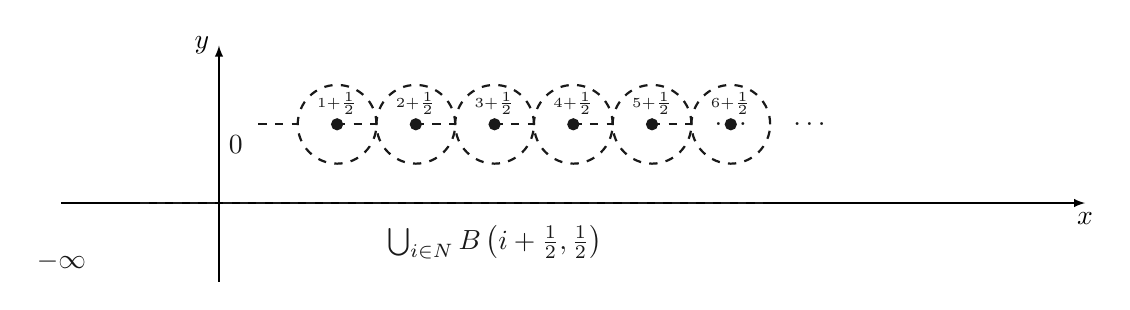
\begin{tikzpicture}
% Eje horizontal
\draw[-latex] (-2,0) -- (11,0) node[below]{$x$};

% Eje vertical
\draw[-latex] (0,-1) -- (0,2) node[left]{$y$};

% Intervalo (-\infty,0)
\node[black!90,below] at (-2,-0.5) {$-\infty$};
\node[black!90,above right] at (0,0.5) {$0$};

% Bolas alrededor de los números naturales
\foreach \x in {1,...,6}
{
\draw[thick,black!90,dashed] (\x+0.5,1) circle (0.5);
\filldraw[black!90] (\x+0.5,1) circle (2pt) node[font=\tiny, above] {\x$+\frac{1}{2}$};
}

% Unión de bolas
\draw[thick,black!90,dashed] (0.5,1) -- (1,1) (1.5,1) -- (2,1) (2.5,1) -- (3,1) (3.5,1) -- (4,1) (4.5,1) -- (5,1) (5.5,1) -- (6,1) (-1,0) -- (7,0);
\node[black!90] at (6.5,1) {$\ldots$};
\node[black!90] at (3.5,-0.5) {$\bigcup_{i\in\mathbb{N}} B\left(i+\frac{1}{2},\frac{1}{2}\right)$};
\node[black!90] at (7.5,1) {$\ldots$};

\end{tikzpicture}

\end{basedtikz}

\begin{proof}
    Para ver que los naturales son cerrados con $d_1$, veamos que su complemento es abierto. Observe que:


    $$\displaystyle \mathbb{R}\setminus\mathbb{N}=(-\infty,0)\bigcup_{i \in \mathbb{N}}B\left(i+\frac{1}{2},\frac{1}{2}\right)$$


Note que esas bolas son abiertas y unión arbitraria de abiertos es abierto, efectivamente esas bolas cubren $\mathbb{R}\setminus \mathbb{N}$ entonces acabamos.
    
\end{proof}


\item[✎]\textbf{Verdadero: } \\
\begin{proof}
    Sea $X\subseteq R$ en $(R,d_d)$, $X$ es abierto ya que:

    $$X=\bigcup_{x \in X}B\left(x,\frac{1}{2}\right)$$

    Y $\mathbb{R}\setminus X$ también ya que:

     $$\mathbb{R}\setminus X=\bigcup_{j \in \mathbb{R}\setminus X}B\left(j,\frac{1}{2}\right)$$

     Luego $X$ es cerrado ya que su complemento es abierto, estos conjuntos los llamaremos \textbf{clopen} para simplificar en algunos casos.
\end{proof}

Note que podemos escoger cualquier $r\leq 1$ y la prueba se mantiene.

\item[✎] \textbf{Falso: }Queremos ver que $[0,\frac{1}{4})^C=[\frac{1}{4},\frac{1}{2})$ no es abierto, note que $B(\frac{1}{4},r)=(\frac{1}{4}-r,\frac{1}{4}+r)$ para todo $r>0$ no está contenida en $[\frac{1}{4},\frac{1}{2})$, entonces $[0,\frac{1}{4})$ no es cerrado en $([0,\frac{1}{2}),d|_{[0,\frac{1}{2})\text{x}[0,\frac{1}{2})})$ 

\item[✎] \textbf{Falso: }El conjunto $\left[0, \frac{1}{2}\right)$ es abierto en $\left(\left[0, \frac{1}{2}\right),\left.d_1\right|_{\left[0, \frac{1}{2}\right) \times\left[0, \frac{1}{2}\right)}\right)$, pero no en $(R,d_1)$

\item[✎]\textbf{Verdadero: }\\
\begin{proof}
    Sea $A$ abierto en $(E,d)$, entonces:

    $$A=\bigcup_{a\in A} B(a,r_a)$$

    Luego:

    $$A\cap E_1=\bigcup_{a\in A} B(a,r_a)\cap E_1$$

Y sabemos que $B(a,r_a)\cap E_1$ es abierto en $E_1$ y como unión arbitraria de abiertos es abierto $A\cap E_1$ es abierto, es decir $A$ es abierto en $E_1$.\\
\end{proof}

Y acabamos esta sección.
\end{itemize}


\section{Quiz 5: }

\begin{itemize}[leftmargin=*]
    \item[✎]\textbf{Verdadero: }\\
    \begin{proof}
        Sea $x \in \mathbb{R}$ entonces $(B(x,\frac{1}{3})\setminus \{x\})=\text{\O}$, luego $(B(x,\frac{1}{3})\setminus \{x\})\cap \mathbb{Q}=$\O, por tanto $\mathbb{Q}^{\prime}=$\O.\\ 
    \end{proof}


    \item[✎] \textbf{Falso: }Sabemos que $S$ es cerrado si y solo si $\overline{S}=S$, antes probamos que $\mathbb{N}$ en $(\mathbb{R},d_1)$ es cerrado luego $$\overline{\mathbb{N}}=\mathbb{N}$$


    \item[✎] \textbf{Falso: }Sabemos que $\partial \mathbb{Q}=$$\overline{\mathbb{Q}}\cap$$\overline{\mathbb{R}\setminus\mathbb{Q}}$ y como $\mathbb{Q}$ y $\mathbb{R}\setminus\mathbb{Q}=\mathbb{I}$ son densos en $\mathbb{R}$ entonces $\overline{\mathbb{Q}}=\mathbb{R}$ y $\overline{\mathbb{I}}=\mathbb{R}$, así $\partial \mathbb{Q}=\mathbb{R}$


    \item[✎] \textbf{Verdadero: }\\
    \begin{proof}
        Tenemos que $x \in [0,1)^{\prime}$ si y solo si $x \in \overline{[0,1)-\{x\}}$, observe que:
        
        \begin{align*}
            \overline{[0,1)-\{x\}}&=[0,1)\setminus int([0,1]\setminus ([0,1)\setminus \{x\}))\\
            &=[0,1)\setminus int(\{x\})\\
            &=[0,1)\setminus \text{\O}
        \end{align*}
        
        En efecto si $x\in [0,1)$, $x \in [0,1)^{\prime}$ 
    \end{proof}

    \item[✎]\textbf{Verdadero: }$\partial \mathbb{R}=$$\overline{\mathbb{R}}\cap$$\overline{\text{\O}}=\mathbb{R}\cap$\O$=$\O


    \item[✎]\textbf{Verdadero: } \\
    \begin{proof}
        Como en las pruebas anteriores note que si $r\leq1$ entonces para todo $x\in \mathbb{R}$, $B(x,r)\setminus\{x\}=$$\emptyset$ y por tanto $B(x,r)\setminus\{x\}\cap \mathbb{R}=$\O, luego $\mathbb{R}^{\prime}=$\O
    \end{proof}


    \item[✎] \textbf{Falso: }Sea $(\mathbb{R},d_d)$ los reales con la métrica discreta, luego:

    $$\overline{B(0,1)}=\overline{\{0\}}=\{0\}$$

Mientras que:

$$B[0,1]=\mathbb{R}$$

    \item[✎]\textbf{Verdadero: }\\
    \begin{proof}
        Tenemos que: 

    $$
d_1(p, q)=\sum_{k=1}^n\left|p_k-q_k\right|
$$
$y$
$$
d_{\infty}(p, q)=\operatorname{máx}_{1 \leq k \leq n}\left|p_k-q_k\right| .
$$

Pero como en este caso estamos en $\mathbb{R}$, entonces 

$$
d_1(p, q)=|p-q|=d_{\infty}(p,q)
$$

Entonces como $\mathbb{N}$ es cerrado en $(\mathbb{R},d_1)$, también es cerrado en $(\mathbb{R},d_{\infty})$

    \end{proof}

    \item[✎]\textbf{Verdadero: }\\
    
   \begin{proof}
         Tenemos que $A$ es cerrado en $(\mathbb{R}^n,d_{\infty})$, luego $A^C$ es abierto en $(\mathbb{R}^n,d_{\infty})$, así para todo $x\in A^C$ existe un $r_x$ tal que:

         $$B_{\infty}(x,r_x)=\{y\in \mathbb{R}^n: d_{\infty}(x,y)<r_x\}\subseteq A^C$$

         Ahora supongamos que $A$ no es cerrado en $(\mathbb{R}^n,d_1)$, luego $A^C$ no es abierto en $(\mathbb{R}^n,d_1)$, es decir, existe $a \in A^C$ tal que para todo $r>0$:

         $$B_2(a,r)\not \subseteq A^C$$

         En particular $B_2(a,r_a)\not \subseteq A^C$, pero como $d_{\infty}(x,y)\leq d_2(x,y)<r_a$, entonces $B_2(a,r_a)\subseteq B_{\infty}(a,r_a)\subseteq A^C$, contradicción.
         
    \end{proof}
    
   

    
\end{itemize}
\vspace{0.3cm}
 \section{Ejercicios adicionales.}
    
\begin{note}
 los siguientes ejercicios fueron propuestos en 2022-2 en un parcial de Análisis, el propósito de esta sección es que sirva para que el estudiante pueda hacerse una idea del modelo de preguntas que se suelen hacer y esté preparado
\end{note}


\begin{itemize}[leftmargin=*]

\item[]\textbf{En cada caso determine si el enunciado es verdadero o falso. Si es verdadero demuéstrelo de lo contrario dé un contra ejemplo.}

    \item[☠]Si $A \neq \varnothing$ es un subconjunto cerrado y acotado inferiormente en $\mathbb{R}$ con la métrica usual $|x-y|$ entonces $A$ tiene elemento mínimo.\\
    
    \textbf{Verdadero:}\\
    
    \begin{proof}
        Supongamos que $A$ es acortado inferiormente en $\mathbb{R}$, entonces existe $i=\inf(A)$, veamos que $i\in A$. Supongamos que $i \not \in A$, entonces $i \in \mathbb{R}\setminus A$, $\mathbb{R}\setminus A$ es abierto porque $A$ es cerrado, entonces existe $\epsilon>0$ tal que $B(i,\epsilon)=(i-\epsilon,i+\epsilon)\subseteq \mathbb{R}\setminus A$, por otro lado como $i=\inf(A)$ existe $b\in A$ tal que $i\leq b< i+\epsilon$, luego $b\in (i-\epsilon,i+\epsilon)\subseteq \mathbb{R}\setminus A$. Contradicción, luego $i \in A$, es decir $i=\min(A)$.
        
    \end{proof}
    
    \item[☠]Sean $(X, d)$ un espacio métrico y $A, B$ subconjuntos de $X$ tales que $int($$A) \subseteq B \subseteq \bar{A}$ entonces $\bar{B}=\bar{A}$.\\
    
    \textbf{Falso: }Contraejemplo: Sean $(\mathbb{R},d_1)$, $\mathbb{N}=A$ y $\{0\}=B$, entonces como $int(\mathbb{N})=$\O, es claro que $int(\mathbb{N})\subseteq\{0\}$, por otro lado $\overline{\mathbb{N}}=\mathbb{N}$ ya que $\mathbb{N}$ es cerrado, y $\overline{\{0\}}=\{0\}$, en efecto $\{0\}\neq \mathbb{N}$.
    
    \item[☠]Si $(X, d)$ es un espacio métrico entonces $d^{\prime}(x, y)=d^2(x, y)$ también define una métrica en $X^2$.
    
    \textbf{Falso: }Contraejemplo: Tome $(\mathbb{R},d_1)$, veamos que $(\mathbb{R},d_1^2)$ no es un espacio métrico. Note que $d_1^2(3,1)>d_1^2(3,2)+d_1^2(2,1)$ $(4>1+1)$, lo que contradice la desigualdad triangular
    
    \item[☠]$(X, d)$ un espacio métrico y $\left(A_j\right)_{j \in J}$ una familia de subconjuntos de $X$. Si $a \in \overline{A_j}$ para todo $j \in J$ entonces $a \in \overline{\bigcap_{j \in J} A_j}$.\\
    
    \textbf{Falso: }Contrajemplo: Sean $\mathbb{Q}, \mathbb{I}$, en $(\mathbb{R},d_1)$, y sea $x=\sqrt{2}$, como $\overline{\mathbb{Q}}=\overline{\mathbb{I}}=\mathbb{R}$, $x \in \overline{\mathbb{Q}}$ y $x\in \overline{\mathbb{I}}$, sin embargo $x\not \in \overline{\mathbb{Q}\cap \mathbb{I}}=\overline{\text{\O}}=$\O

    
    \item[☠☠] Sean:
    \begin{itemize}
        
\item $X$ el espacio de las funciones acotadas $f: I \rightarrow \mathbb{R}$ definidas en el intervalo real $I=[0,1]$,

\item $d$ la métrica definida en $X^2$ por $d(f, g)=\sup _{x \in I}|f(x)-g(x)|$,

\item $f_0(x)=x^2, f_n(x)=\dfrac{x^2 \operatorname{sen}(2 \pi n x)}{2 \pi n}                       
    \operatorname{con} n \in \mathbb{Z}^{+}, x \in I$ y

\item $B\left(f_0, \frac{3}{2}\right)=\left\{f \in X: d\left(f, f_0\right)<\frac{3}{2}\right\}$
entonces $f_n \in B\left(f_0, \frac{3}{2}\right)$ para todo $n \in \mathbb{Z}^{+}$.\\

    \end{itemize}
   
 \begin{proof}
    Queremos ver que $f_n\in B(f_0,\frac{3}{2})$ para todo $n \in \bb{Z}^+$, es decir que $d(f_n,f_0)<\frac{3}{2}$ para todo $n \in \bb{Z}^+$, luego por la definición de la métrica:
    
    \begin{align*}
        d(f_n,f_0)&=\sup_{x \in I}\left|x^2-\dfrac{x^2sen(2\pi nx)}{2\pi n}\right|\\
        &=\sup_{x \in I}\left|x^2\left(1-\dfrac{sen(2\pi nx)}{2\pi n}\right)\right|\\
        &\leq\sup_{x \in I}\left|1-\dfrac{sen(2\pi nx)}{2\pi n}\right| && (x^2\leq 1)\\
        &\leq\left|1-\dfrac{1}{2\pi n}\right|&&(-1\leq sin(\theta)\leq 1)\\
        &\leq \dfrac{3}{2}\\
        &=1.5
     \end{align*}

Ya que $0<\frac{1}{2\pi n}< 1$ para todo $n \in \Z^+$

    
\end{proof}  
   
   \begin{note}
   cuando decimos métrica sobre $X^2$ queremos decir que la métrica va del producto cartesiano $X \text{ x } X$ en $\bb{R}$, no confundir con $X^2 \text{ x } X^2$ 
   \end{note}
   


\begin{note}
Los siguientes ejercicios fueron propuestos en 2023-1 en el primer parcial de análisis:
\end{note}

\end{itemize}


Sean $(X, d)$ es un espacio métrico y $A$ es un subconjunto de $X$. En cada caso determine si la proposición es verdadera o falsa y demuéstrela o dé un contra-ejemplo según sea el caso.

\begin{itemize}[label={☠},leftmargin=*]
\item $X=\overline{A}\cup A^{C}$\\

\begin{proof}
Sabemos que $\overline{A}=X\setminus int(A^C)$. En efecto $X\setminus int(A^C)\cup A^C=X$ ya que $int(A^C)\subseteq A^C$
\end{proof}
 
\item $\partial(\partial A)=\partial A$\\

\textbf{Falso:} Contraejemplo: Considere $(\R,d_1)$, sabemos que $\partial \Q=\R$ y que $\partial \R= $\O, luego $\partial \Q=\R\neq\partial(\partial \Q)=\partial \R=$\O

\item $X=int(A)\cup \partial(A) \cup A^C$\\

\begin{proof}
Tenemos que $\partial A=\bar{A} \cap \overline{A^C}$, luego

\begin{align*}
int(A)\cup (\overline{A}\cap \overline{A^C}) \cup A^C&=int(A)\cup (\overline{A}\cup A^C\cap \overline{A^C}\cup A^C)\\
&=int(A)\cup (X\cap (X\setminus int(A)\cup A^C))\\
&=int(A)\cup (X\setminus int(A))\\
&=X
\end{align*}
\end{proof}

\begin{note}
Aquí usamos varias de las propiedades de las notas en el capítulo del concepto de clausura, derivado y frontera, note que además usamos la propiedad anterior en la prueba cuando afirmamos que $\overline{A}\cup A^C=X$, note también que usamos que $(A^C)^C=A$ pero pues ustedes ya vieron conjuntos allí.
\end{note}

\item $int(int(A))=int(A)$\\

\begin{proof}
 Tenemos que $int(A)$ es abierto, luego como un conjunto es abierto si y solo si es igual a su interior entonces $int(int(A))=int(A)$
\end{proof}


\item Si $\partial A$ es abierto entonces $A=$\O\\

\textbf{Falso:} Contraejemplo: Considere $(R,d_1)$, luego $\partial \Q=\R$ y $\R$ es abierto pero $\Q\neq$\O.



\item Si $X=\mathbb{R}^n$ y $A$ es $d_1$-abierto entonces $A$ es $d_2$-abierto.\\

\begin{proof}
Suponga que $A$ es $d_1$-abierto, entonces para todo $x\in A$, existe $r$ tal que:
 
$$B_1(x,r)=\{y\in \R^{n} : d_1(x,y)<r\}\subseteq A$$

Y como $d_2(x,y)\leq d_1(x,y)$, entonces existe $r^{\prime}$ $B_2(x,r^{\prime})\subseteq B_1(x,r)\subseteq A$, luego $A$ es $d_2-$abierto

\end{proof}

\begin{note}
Para este caso estamos usando la definición de métrica equivalente, note que si $d_2(x,y)\leq d_1(x,y)$ entonces existe $C\in \R$ tal que $d_1(x,y)\leq C d_2(x,y)$, luego eso es lo que nos garantiza la existencia de ese radio $r^{\prime}$ de tal manera que $B_2(x,r^{\prime})\subseteq B_1(x,r)$. 
\end{note}

\begin{note}
Note que en las notas hace falta hacer énfasis en esta definición, sin embargo este tipo de detalles se suelen cubrir en clase, en cualquier caso el lector puede buscar en algún medio externo la definición de métrica equivalente y notar este detalle sutil.
\end{note}



\item Si $A \subseteq Y \subseteq X$ y $A$ es $Y$-abierto entonces $A$ es $X$-abierto.\\

\textbf{Falso: } Contraejemplo: Si $E=\mathbb{R}$ con $d(x, y)=|x-y|$ el conjunto $\left[0, \frac{1}{3}\right)$ no es abierto en $\mathbb{R}$ pero es abierto en $\left(E_1,\left.d\right|_{E_1 \times E_1}\right)$ con $E_1=\left[0, \frac{1}{2}\right)$. Simplemente observe que $B_{E_1}\left(0, \frac{1}{3}\right)=\left[0, \frac{1}{3}\right)$.

\item Si $x \in X$ entonces para todo $r>0$ se tiene que $\overline{B(x, r)}=B[x, r]$.\\

\textbf{Falso:} Contraejemplo: Sea $(\R,d_d)$, entonces $\overline{B(0,1)}=\overline{\{0\}}=0$ ya que $\{0\}$ es cerrado con la métrica discreta, pero $B[0,1]=\R$, luego no son iguales.

\end{itemize}

\begin{note}
Sobre este parcial como se puede notar los ejercicios no son tan complejos si se nos permite usar las propiedades de las notas (que se ven también en clase), pero es probable que para ser usadas en el parcial el estudiante deba demostrarlas, en cuyo caso recomendamos entender muy bien las ideas de cada una de las pruebas, la idea nunca es memorizar las pruebas o las propiedades sino entender un poco la geometría del asunto y las ideas principales de cada prueba.
\end{note}

\section{El conjunto de Cantor ☠☠☠☠☠}

\begin{note}
En esta sección solo trataremos el problema de probar que el conjunto de cantor es perfecto, es decir que todo elemento del conjunto pertenece a su derivado. Quizás luego pongamos un diagrama de la prueba de que no es contable, un resultado más fuerte que quizás se podría sugerir es revisar la prueba de que todo conjunto perfecto no puede ser contable.
\end{note}

\begin{itemize}[label={✎},leftmargin=*]

\item El conjunto de Cantor es perfecto:\\


\begin{proof}
Para demostrar que el conjunto de Cantor $C$ es perfecto, para cada $x \in C$ y para cada $\epsilon>0$ se debe encontrar un punto $y \in C-\{x\}$ tal que $|x-y|<\epsilon$.

Para buscar $y$, recordemos que $C$ se construye como la intersección de conjuntos $C_0 \supset C_1 \supset C_2 \supset C_3 \supset \cdots$ donde $C_n$ es una unión de $2^n$ intervalos disjuntos cada uno de longitud $3^{-n}$, y recordemos también que $C$ tiene intersección no vacía con cada uno de esos $2^n$ intervalos.

Elija $n$ tal que $3^{-n}<\epsilon$.
Sea $[a, b]$ el intervalo de $C_n$ que contiene a $x$.
Cuando se quita el tercio medio de $[a, b]$, se obtienen dos intervalos $\left[a, b^{\prime}\right],\left[b^{\prime \prime}, b\right]$ de $C_{n+1}$. El punto $x$ está contenido en uno de esos dos intervalos, y hay un punto $y \in C$ que está contenido en el otro de esos dos intervalos. Por lo tanto, $y \neq x$ y $|x-y|<\epsilon$.
\end{proof}

\begin{note}
        Enlace para ver la prueba de que todo conjunto perfecto no es contable: 

        \href{https://math.stackexchange.com/questions/201922/proof-that-a-perfect-set-is-uncountable}{\textcolor{blue}{Enlace.}} 
\end{note}

\item El conjunto de Cantor es no contable
        
\end{itemize}

\section{Sucesiones ☠☠☠☠☠}

Este capítulo es cosa densa, mucho cuidado.

\subsection{Algunos ejercicios al lector:}

En esta sección también hay algunos ejercicios que el libro dice que son triviales,pero lo que es trivial hay que demostrarlo.

\begin{itemize}[label={✎},leftmargin=*]

\item Es fácil demostrar que $n_k\geq k$ (Inducción)

\begin{proof}
Supongamos que la secuencia comienza en $k=1$. Entonces, lo más pequeño que puede ser $n_1$ es 1. Por lo tanto, $n_k \geq k$ es verdadero para $k=1$. Ahora, asumimos por inducción que $n_k \geq k$ para algún $k$. Dado que lo más pequeño que puede ser $n_{k+1}$ es $n_k+1$, obtenemos
$$
n_{k+1} \geq n_k+1 \geq k+1.
$$
\end{proof}

(Para esta prueba es clave saber que tanto $k$ como $n_k$ son naturales.)

\begin{note}
Note que una subsecesión podría verse como un subconjunto de una sucesión ya que los puntos $\{x_{n_1},x_{n_2},\ldots\}\subseteq\{x_1,x_2,\ldots\}$. Esto es lo que nos permite ver que toda subsucesión de una sucesión acotada es acotada.


\end{note}

\begin{note}
En el teorema 10 lo que nos quieren decir es que $S\subseteq E$ es cerrado si y solo si cualquier sucesión convergente en el espacio que es definida en $S$ converge en $S$, o sea su límite pertenece a $S$, algo de esperar.
\end{note}


\item En la proposición 22 se hace la prueba para sucesiones crecientes pero no decrecientes, veamos ese caso:\\

\begin{proof}
Sea $(a_n)_{n  \in \N}$ una sucesión decreciente y acotada en $(\R,d_1)$, como $(a_n)_{n\in \N}$ es acotada entonces es acotada inferiormente y por lo tanto existe $I=\inf\{a_n: n\in \N\}$. Veamos que el $\lim_{n\to \infty}a_n=I$. Dado $\epsilon>0$ por la propiedad de aproximación existe $N\in \N$, tal que $I+\epsilon>a_N$ y como $(a_n)_{n\in \N}$ es decreciente

$$I+\epsilon>a_N\geq a_n\quad \text{si }n \geq N$$

Por otro lado $I+\epsilon>a_n>I-\epsilon$ (ya que $I=\inf\{a_n: n\in \N\}$), Así $|a_n-I|<\epsilon$ para todo $n\geq N$, luego $\lim_{n\to\infty}a_n=I$
\end{proof}

\item Ejercicio proposición 23\\

\begin{theorem}{Proposición 23:}

Sean $(a_n)_{n\in \N}$ y $(b_n)_{n\in \N}$ sucesiones en $(\R,d_1)$, si $(a_n)_{n\in \N}$ y $(b_n)_{n \in \N}$ son convergentes, entonces:

\begin{itemize}
    \item $(a_n\pm b_n)_{n\in \N}$ es convergente y $\lim_{n \to \infty}(a_n\pm b_n)=\lim_{n \to \infty} a_n\pm \lim_{n \to \infty} b_n $
\end{itemize}
\end{theorem}

\begin{lemma}
Si $(b_n)_{n\in \N}$ es una sucesión convergente (que converge a $b$), entonces $(-b_n)_{n\in \N}$ es convergente y converge a $-b$.
\end{lemma}

\begin{proof}
Tenemos que $(b_n)_{n\in \N}$ es convergente y converge a $b$, es decir para todo $\epsilon>0$ existe $N\in \N$ tal que si $n>N$ $|b_n-b|<\epsilon$, luego:

$$|-b_n+b|=|-1(b_n-b)|=|-1||b_n-b|=|b_n-b|<\epsilon$$

Luego $(-b_n)_{n\in\N}$ es convergente y converge a $-b$
\end{proof}

Con este lema podemos hacer la prueba del teorema solo para $((a_n)_{n\in \N}+(b_n)_{n\in \N})_{n\in \N}$ ya que el caso de la resta es corolario de esto, note que basta considerar la sucesión $(-b_n)_{n\in \N}$ y usar el resultado para la suma.

\begin{proof}
    Tenemos que $(a_n)_{n\in N}$ y $(b_n)_{n\in \N}$ son convergentes, es decir para todo $\epsilon>0$ existen $N_1\in \N$ y $N_2\in \N$ tales que si $n>N_1$ $|a_n-a|<\frac{\epsilon}{2}$ y si $n>N_2$, $|b_n-b|<\frac{\epsilon}{2}$, luego si $n>\max\{N_1,N_2\}$, entonces.

    $$|a_n+b_n-a-b|\leq |a_n-a|+|b_n-b|=\frac{\epsilon}{2}+\frac{\epsilon}{2}=\epsilon$$
\end{proof}

\begin{note}
En estas pruebas siempre al escribirlas debemos saber las cotas que vamos a usar, pero esto no significa que siempre debamos ver a ojo que cota usar, usando la definición nos hubiéramos dado cuenta que la suma de las cotas nos iba a dar $2\epsilon$, por eso escogemos $\frac{\epsilon}{2}$, porque queremos que la suma sea menor que $\epsilon$, en análisis esto se hace para que las demostraciones tengan un mejor estilo, escritura y forma, se supone que con práctica el estudiante debería ser capaz de ver algunas de estas cotas sin mucho esfuerzo, pero si esto no se te da bien no te preocupes, a mí tampoco.
\end{note} 

Recordemos que en este punto estamos trabajando con los REALES, ya que vamos a comenzar con el capítulo de límite superior e inferior.


\subsection{Límite superior y límite inferior:}

Esta sección puede resultar confusa en un inicio, aquí trataremos de desglosar un poco la idea fundamental de todo.

\begin{basedtikz}


\tikzset{every picture/.style={line width=0.75pt}} %set default line width to 0.75pt        

\begin{tikzpicture}[x=0.75pt,y=0.75pt,yscale=-1,xscale=1.5]
%uncomment if require: \path (0,472); %set diagram left start at 0, and has height of 472

%Curve Lines [id:da44573902991754766] 
\draw  [dash pattern={on 0.84pt off 2.51pt}]  (141.52,165.81) .. controls (164.19,155.81) and (164.19,308.48) .. (178.57,308.29) .. controls (192.95,308.1) and (201.52,180.48) .. (216.57,178.29) .. controls (231.62,176.1) and (232.95,316.76) .. (249.57,297.29) .. controls (266.19,277.81) and (258.19,196.48) .. (272.57,191.29) .. controls (286.95,186.1) and (272.29,282.77) .. (296.19,281.81) .. controls (320.09,280.85) and (313.07,223.21) .. (320.07,211.71) .. controls (327.07,200.21) and (328.62,283.28) .. (345,281) .. controls (361.38,278.72) and (358.07,222.21) .. (365.07,211.71) .. controls (372.07,201.21) and (375.37,284.12) .. (388.19,281.14) .. controls (401.01,278.16) and (398.57,221.71) .. (405.07,212.21) .. controls (411.57,202.71) and (413.52,290.14) .. (425.52,281.14) .. controls (437.52,272.14) and (431.57,231.21) .. (439.57,213.21) .. controls (447.57,195.21) and (453.65,285.77) .. (462.19,281.14) .. controls (470.73,276.52) and (465.52,219.81) .. (485,211) ;
%Straight Lines [id:da2292557377025013] 
\draw  [dash pattern={on 4.5pt off 4.5pt}]  (120.19,281.14) -- (498.86,280.48) ;
%Straight Lines [id:da021754386863272357] 
\draw  [dash pattern={on 4.5pt off 4.5pt}]  (119.52,210.48) -- (500.19,209.81) ;
%Straight Lines [id:da9184013042125718] 
\draw [color={rgb, 255:red, 208; green, 2; blue, 27 }  ,draw opacity=1 ]   (119.57,165.21) -- (148,165.21) -- (155.6,178.17) -- (221.57,178.21) -- (225.64,191.21) -- (278.14,191.21) -- (280.64,209.71) -- (322.19,209.81) ;
%Straight Lines [id:da2894532143841366] 
\draw [color={rgb, 255:red, 208; green, 2; blue, 27 }  ,draw opacity=1 ]   (120.8,309.77) -- (184,309.85) -- (187.02,299.72) -- (252.4,300.17) -- (258,280.97) -- (293.2,281.37) ;
%Straight Lines [id:da09981137612794089] 
\draw    (228.95,146.57) -- (201.73,172.52) ;
\draw [shift={(200.29,173.9)}, rotate = 316.36] [color={rgb, 255:red, 0; green, 0; blue, 0 }  ][line width=0.75]    (7.65,-2.3) .. controls (4.86,-0.97) and (2.31,-0.21) .. (0,0) .. controls (2.31,0.21) and (4.86,0.98) .. (7.65,2.3)   ;
%Straight Lines [id:da7736001528911756] 
\draw    (240.95,147.9) -- (239.69,183.91) ;
\draw [shift={(239.62,185.9)}, rotate = 272.01] [color={rgb, 255:red, 0; green, 0; blue, 0 }  ][line width=0.75]    (7.65,-2.3) .. controls (4.86,-0.97) and (2.31,-0.21) .. (0,0) .. controls (2.31,0.21) and (4.86,0.98) .. (7.65,2.3)   ;
%Straight Lines [id:da01875292146375851] 
\draw    (223.62,137.9) -- (140.23,158.75) ;
\draw [shift={(138.29,159.24)}, rotate = 345.96] [color={rgb, 255:red, 0; green, 0; blue, 0 }  ][line width=0.75]    (7.65,-2.3) .. controls (4.86,-0.97) and (2.31,-0.21) .. (0,0) .. controls (2.31,0.21) and (4.86,0.98) .. (7.65,2.3)   ;
%Straight Lines [id:da685154290163863] 
\draw    (212.95,355.9) -- (152.67,319.6) ;
\draw [shift={(150.95,318.57)}, rotate = 31.05] [color={rgb, 255:red, 0; green, 0; blue, 0 }  ][line width=0.75]    (7.65,-2.3) .. controls (4.86,-0.97) and (2.31,-0.21) .. (0,0) .. controls (2.31,0.21) and (4.86,0.98) .. (7.65,2.3)   ;
%Straight Lines [id:da47753478631845336] 
\draw    (236.29,347.9) -- (217.17,309.03) ;
\draw [shift={(216.29,307.24)}, rotate = 63.81] [color={rgb, 255:red, 0; green, 0; blue, 0 }  ][line width=0.75]    (7.65,-2.3) .. controls (4.86,-0.97) and (2.31,-0.21) .. (0,0) .. controls (2.31,0.21) and (4.86,0.98) .. (7.65,2.3)   ;
%Shape: Rectangle [id:dp6544720458561455] 
\draw  [dash pattern={on 4.5pt off 4.5pt}] (118.95,126.57) -- (502.29,126.57) -- (502.29,366.57) -- (118.95,366.57) -- cycle ;

% Text Node
\draw (418,194.3) node [anchor=north west][inner sep=0.75pt]  [font=\scriptsize]  {$\limsup x_{n}$};
% Text Node
\draw (420.67,288.3) node [anchor=north west][inner sep=0.75pt]  [font=\scriptsize]  {$\liminf x_{n}$};
% Text Node
\draw (231.33,129.97) node [anchor=north west][inner sep=0.75pt]  [font=\tiny]  {$\sup _{k\geq n} x_{k}$};
% Text Node
\draw (226.67,354.64) node [anchor=north west][inner sep=0.75pt]  [font=\tiny]  {$\inf_{k\geq n} x_{k}$};
% Text Node
\draw (478.14,134.26) node [anchor=north west][inner sep=0.75pt]    {$\mathbb{R}$};


\end{tikzpicture}
\end{basedtikz}



Dada $\left(x_n\right)_{n \in \mathbb{N}}$ acotada en $\mathbb{R}$ existen $\alpha, \beta \in \mathbb{R}$ tales que $\alpha \leq x_n \leq \beta$ para todo $n \in \mathbb{N}$. Si $X_n=\left\{x_k: k \geq n\right\}$ tomamos
$$
\begin{aligned}
& b_n=\sup X_n, \mathrm{y} \\
& a_n=\inf X_n .
\end{aligned}
$$
De esta forma tenemos que
$$
\alpha \leq a_1 \leq a_2 \leq \cdots \leq a_{n-1} \leq a_n \leq \cdots \leq b_n \leq b_{n-1} \leq \cdots \leq b_1 \leq \beta .
$$

\begin{note}
Todo esto se tiene porque primero estamos en los reales y la sucesión es acotada, podemos garantizar el Sup y el Ínf, note que:\\

$$X_1=\{x_1,x_2,\ldots\} \quad \text{y}\quad X_2=\{x_2,x_3,\ldots\}$$

Luego $\sup X_1$ o es $x_1$ o está en $X_2$ y $\sup X_2$ o es $x_2$ o está en $X_3$, luego razonando de esta forma nos damos cuenta que $\sup X_n\leq \sup X_{n-1}$, por eso $b_n\leq b_{n-1}$.
\end{note}

\begin{note}
Todo esto pasa ya que el supremo es mayor o igual que todos los elementos de $X_n$, luego si el supremo de $X_n$ fuera $x_n$, entonces el supremo de $X_{n+1}$ sería más pequeño, y en caso de que no fuera $x_n$, entonces el supremo de $X_n$ y $X_{n+1}$ serían iguales.
\end{note}

Además todos estos $b_n=\sup X_n<\beta$ ya que la sucesión es acotada, para $a_n=\inf X_n$ se razona de la misma forma para llegar a que $a_n\leq a_{n+1}$, espero que esto sea suficiente para entender digamos un poco este tema, es algo que en un inicio cuesta, pero que entenderlo bien es muy muy clave, este tipo de aclaraciones Omar al menos la suele dar en clase, pero en este curso no todos los profesores son tan buenos. 



\begin{definition}
Definimos el límite inferior (denotado por líminf $x_n$ ) y el límite superior (notado por $\left.\operatorname{lím} \sup x_n\right)$ de $\left(x_n\right)_{n \in \mathbb{N}}$ como
$$
\begin{aligned}
& \liminf x_n=\sup a_n=\lim _{n \rightarrow \infty} a_n, \quad y \\
& \lim \sup x_n=\inf b_n=\lim _{n \rightarrow \infty} b_n .
\end{aligned}
$$    
\end{definition}

A continuación presentamos una definición un poco más chingona de límites superior e inferior, son equivalentes en realidad las definiciones, pero esta definición es agradable porque nos evita pensar en $X_n$ y desviar nuestra atención.

\begin{definition}

Definimos el límite inferior (denotado por líminf $x_n$ ) y el límite superior (notado por $\left.\operatorname{lím} \sup x_n\right)$ de $\left(x_n\right)_{n \in \mathbb{N}}$ como:

$$    \begin{aligned}
\lim \inf x_n & =\lim _{n \rightarrow \infty}\left(\inf _{k \geq n} x_k\right) \\
\lim \sup x_n & =\lim _{n \rightarrow \infty}\left(\sup _{k \geq n} x_k\right)
\end{aligned}$$

\end{definition}


\section{Quiz 6:}

\end{itemize}

\begin{itemize}[label={✎},leftmargin=*]
    \item 

    \item Verdadero:\\

    \begin{proof}
    Tenemos que $(a_n)$ es convergente, luego:

    \begin{align*}
        a=\lim_{n \to \infty} a_n&=\lim_{n \to \infty} a_{n+1}\\
        &=2\lim_{n \to \infty}(a_n)^2-\lim_{n \to \infty} a_{n-1}\\
        &=2a^2-a\\
        &=a(2a-1)
    \end{align*}
    
    Entonces $(2a-1)=1$, por tanto $a=1$.
    \end{proof}


    \item Verdadero:\\

    \begin{proof}
    Tenemos que existe $m\in \N$ tal que $a_n=b_n$ para todo $n\geq m$, luego como $a_n$ es convergente, para todo $\epsilon>0$, existe un $N\in \N$ tal que si $n>\max\{N,m\}$, entonces:

    $$|b_n-a|=|a_n-a|<\epsilon$$

    Luego $b_n$ es convergente y además converge a $a$
    \end{proof}

\begin{note}
Usamos el máximo ya si $m$ es el máximo entonces a partir del punto en que $a_n=b_n$ ya tenemos convergencia, si $N$ es el máximo entonces desde antes de tener convergencia ya teníamos que $a_n=b_n$, luego es conveniente escoger $n>\max\{N,m\}$, para que se de $n$ en adelante tengamos tanto convergencia como que las sucesiones son iguales.
\end{note}
    
    \item Falso: Considere $(\R,d_1)$, (note que en $\R$, $d_2=d_1$), entonces si tomamos una sucesión constante, $(x_n)_{n\in\N}=(-1)^na_n$ no converge, por ejemplo: si $(a_n)_{n\in \N}=1$, entonces:

    $$(x_n)_{n\in \N}=\{-1,1,-1,1,-1,1,\ldots\}$$ 

    Vemos que $(x_n)_{n\in\N}$ no converge, para ello veamos que el límite superior no es igual al límite inferior\\

    Note que $\lim_{n \to \infty} \left( \inf_{k\geq n} x_k \right)=\lim_{n \to \infty} -a_n=\lim_{n \to \infty} -1=-1$ y por otro lado el \\
    $\lim_{n \to \infty} \left( \sup_{k\geq n} x_k\right)=\lim_{n \to \infty} a_n=\lim_{n \to \infty} 1=1$

    \item Verdadero:\\ \begin{proof} 
    Observe que para todo $\epsilon>0$, existe $N\in \N$ tal que $\frac{1}{N}<\epsilon$, entonces si $n>N$:


    $$\left| \frac{1}{n} \right|<\epsilon$$

    Luego:

    $$\lim _{n \rightarrow \infty}\left(\sup _{k \geq n} \frac{(-1)^n}{n}\right)$$

    Veamos entonces quien es el $\sup_{k\geq n}\frac{(-1)^n}{n}$.

    \begin{align*}
        &\sup X_2=\sup \left\{\frac{1}{2},-\frac{1}{3},\frac{1}{4},\ldots\right\}\\
        &\sup X_3=\sup\left\{-\frac{1}{3},\frac{1}{4},-\frac{1}{5},\ldots\right\}\\
        &\sup X_4=\sup\left\{\frac{1}{4},-\frac{1}{5},\frac{1}{6},\ldots\right\}\\
        &\sup X_5=\sup\left\{-\frac{1}{5},\frac{1}{6},-\frac{1}{7},\ldots\right\}\\
        & \mathrel{\phantom{=askldfjaddsl}}\vdots
    \end{align*}

    Note que si $n$ es par entonces:

    $$\lim _{n \rightarrow \infty}\left(\sup_{k \geq n} \frac{(-1)^n}{n}\right)=\lim_{n \to \infty} \frac{1}{n}=0$$

    Si $n$ es impar:

    $$\lim _{n \rightarrow \infty}\left(\sup _{k \geq n} \frac{(-1)^n}{n}\right)=\lim_{n \to \infty} \frac{1}{2n+1}=0$$
    
    No es necesario probar este límite ya que probamos el caso general $\frac{1}{n}$ da 0.

    \end{proof} 


    \item Falso: 

        $$\liminf \frac{(-1)^n n}{n+1}=\lim _{n \rightarrow \infty}\left(\inf_{k \geq n} \frac{(-1)^nn}{n+1}\right)$$

        Veamos entonces quién es el $\inf_{k\geq n} \frac{(-1)^nn}{n+1}$:

        \begin{align*}
            &\inf X_1=\inf \left\{-\frac{1}{2},\frac{2}{3},-\frac{3}{4},\ldots\right\}=-1\\
            &\inf X_2=\inf \left\{\frac{2}{3},-\frac{3}{4},\frac{4}{5},\ldots\right\}=-1\\
            &\inf X_3=\inf \left\{-\frac{3}{4},\frac{4}{5},-\frac{5}{6},\ldots\right\}=-1\\
            &\inf X_4=\inf \left\{\frac{4}{5},-\frac{5}{6},\frac{6}{7},\ldots\right\}=-1\\
            &\inf X_5=\inf \left\{-\frac{5}{6},\frac{6}{7},-\frac{7}{8},\ldots\right\}=-1\\
            & \mathrel{\phantom{=askaldfjasl}}\vdots
        \end{align*}

        Luego el $\inf_{k\geq n} \frac{(-1)^nn}{n+1}$ siempre es -1, por tanto:

        $$\liminf \frac{(-1)^n n}{n+1}=\lim _{n \rightarrow \infty}\left(\inf_{k \geq n} \frac{(-1)^nn}{n+1}\right)=\lim_{n \to \infty} -1=-1$$




    \item Verdadero: Primero note que:

    $$\sqrt{n+1}-\sqrt{n} \left(\frac{\sqrt{n+1}+\sqrt{n}  }{\sqrt{n+1}+\sqrt{n} } \right)=\frac{1}{\sqrt{n+1}+\sqrt{n}}<\frac{1}{2\sqrt{n}}$$


    \begin{proof}
    
    Para todo $\epsilon>0$ existe un  $N\in  \N$ tal que $N>\frac{1}{4\epsilon^2}$, luego si $n>N$:

        $$\left|\frac{1}{2\sqrt{n} }\right|<\left|\frac{1}{2\sqrt{N} }\right|<\left|\frac{1}{2\sqrt{\frac{1}{4\epsilon^2}} }\right|=\epsilon$$


Luego en efecto $\lim_{n \to \infty} \sqrt{n+1}-\sqrt{n}=0   $
    \end{proof}

    

    \item Falso: Contraejemplo: Sea $A=\{(x,e^x) : x\in \R\}$ y $B=\{(y,0): y\in \R\}$, luego note que $\overline{B}=B$ y $\overline{A}=A$.

    $$A+B=\{(z,e^w): z,w\in \R\}=\{(x,y): x,y\in \R, y>0 \}$$

    Luego $\overline{A+B}=\{(x,y):x,y\in \R,y\geq0\}\neq\overline{A}+\overline{B}$



\end{itemize}


\section{Completez}

\subsection{Algunos ejercicios al lector}

\begin{itemize}[label={✎},leftmargin=*]
    \item Si $(x_n)$ es una sucesión convergente, entonces $(x_n)$ es una sucesión de Cauchy.

    \begin{proof}
    Sea $(x_n)$ una sucesión convergente, entonces para todo $\epsilon>0$, existe $N\in \N$ tal que si $n,m>N$, entonces $d(x_n,L)<\frac{\epsilon}{2}$ y $d(x_m,L)<\frac{\epsilon}{2}$. Así:

    $$d(x_n,x_m)\leq d(x_n,L)+d(L,x_m)<\frac{\epsilon}{2}+\frac{\epsilon}{2}=\epsilon$$
    \end{proof}

    \item Si $(x_n)$ es una sucesión de Cauchy, entonces toda subsucesión también es de Cauchy.

    \begin{proof}
        Sea $(x_n)$ una sucesión de Cauchy, entonces para todo $\epsilon>0$, existe $N\in \N$ tal que si $m,n\geq N$, $d(x_n,x_m)<\epsilon$.\\

        Considere $(x_{n_k})$ una subsucesión de $(x_n)$, luego como $n_k\geq k$, para todo $k\in \N$, en efecto si $L,M\geq k\geq N$ entonces $n_L,n_M\geq N$ y como $(x_n)$ es de Cauchy:

        $$d(x_{n_L},x_{n_M})<\epsilon$$ 
    \end{proof}
\end{itemize}

\section{Quiz 7}

\begin{itemize}[label={✎},leftmargin=*]
    \item Verdadero:\\

    \begin{proof}
        Sea $(x_n)$ una sucesión de Cauchy en $(\Z,d_1)$, luego para todo $\epsilon>0$, existe $N\in \N$ tal que si $n,m\geq N$, entonces:

        $$|x_n-x_m|<\epsilon$$

        Por tanto $x_n=x_m$, es decir $(x_n)$ es constante, entonces $\lim_{n \to \infty} x_n=x_m$, como $x_m \in \Z$, acabamos.
    \end{proof}

    \item Verdadero: veamos un resultado más elegante. Sea $(X,d_d)$ donde $d_d$ es la métrica discreta, entonces $X$ es completo.\\

    \begin{proof}
        Sea $(x_n)$ una sucesión de Cauchy en $(X,d_d)$, entonces para todo $\epsilon>0$, existe $N\in\N$ tal que si $m,n\geq N$, entonces:

        $$d_d(x_n,x_m)<\epsilon$$

        Sea $\epsilon=\frac{1}{2}$, entonces:

        $$d_d(x_n,x_m)<\frac{1}{2}$$

        Entonces $x_n=x_m$, luego $(x_n)$ es constante, por tanto converge en $X$.
    \end{proof}

    \item Verdadero:\\

    \begin{proof}
        Considere $(x_n)=\left( 1+\frac{1}{n} \right)^n$, esta sucesión es de Cauchy en $\Q$, es fácil ver que:

        $$\lim_{n \to \infty} \left( 1+\frac{1}{n} \right)^n=e$$

        Ejercicio: Pruebe que $e$ no es racional.
    \end{proof} 

    \item Verdadero:\\ 

    \begin{proof}
        Sabemos que $(\R^m,d_2)$ es completo, luego si $(a_n)$ es de Cauchy, entonces es convergente, tenemos que $(b_n)$ es convergente, por tanto $(a_n+b_n)$ es convergente, y toda sucesión convergente es de Cauchy.
    \end{proof}

    \item Verdadero:\\

    \begin{proof}
        Sabemos que $(R^m,d_2)$ es completo, luego si $(x_n)$ es una sucesión de Cauchy en $(\R^m,d_2)$, para todo $\epsilon>0$, existe $N\in \N$ tal que si $n>N$:

        $$d_2(x_n,L)\leq \epsilon$$

        Luego como $d_{\infty}(x,y)\leq d_2(x,y)$:

        $$d_{\infty}(x_n,L)\leq d_2(x_n,L)<\epsilon$$

        i.e. $(\R^m,d_{\infty})$ es completo.
    \end{proof}
\end{itemize}

